\subsection{Requirements gathering methodology}

In a systems development, understanding the customer�s way of thinking, expectation and basic needs is the first major task any systems developer tackle. Understanding a customer saves time, results in happier customer, better reputation, and boosts developer productivity. Employing the right requirements capturing methodology and strict follow up of gathered requirements should in general keep customers and developers on the same page. Requirements gathering technique, if applied accurately, will serve as a suitable preemptive action against fluid, incomplete, constantly evolving requirements, and force both parties hold fast to, in addition, the legal and contractual agreements between a customer and a developer. Here is a list of industry proven of requirements capturing techniques.

\subsubsection{Background reading}

A developer can understand the internal operations, services and cooperation of a company by reading about the background of the organization. Specialized tasks, projects, cultures and improvement requiring sides are to be investigated by reading company reports, organizational charts, policy manuals, job description and documentation of an existing system.

\subsubsection{Interviewing and questionnaires}

System analyst interviews the personnel of an organization to understand how they accomplish their day to day activity. It is very advantageous to gather firsthand information about priorities, objectives and required improvements for the system in perspective of all stake holders�including workers and management involved. Even though the quality information gather from an interview can be invaluable, it has a tendency to go off topic and extremely expensive. Questionnaires can be an alternative way of providing a goal oriented investigation about an operation of existing system, and to find out current satisfaction, improvement suggestions.

\subsubsection{Observation and document sampling}

Observation and document sampling is a technique effective to capture requirements that are impossible to understand through interviews and
questionnaires. It will also enable analysts to gather quantitative data on how long a task takes to complete in real time. However, observation can be problematic requirements that involve sensitive information such as private data, medical, education and other protected information.
\subsection{MOWAHS Requirement Analysis Framework}
The MOWAHS, MObile Work Across Heterogeneous Systems, a specialized technique to analyze gathered requirements for mobile work scenario.  The framework has three levels of operation eliciting scenarios, scenario analysis and requirement analysis.

\begin{figure}[htb]
	\centering
	 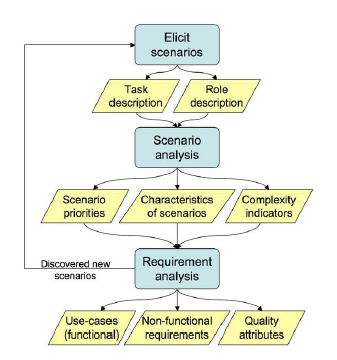
\includegraphics[width=0.8\textwidth]{prestudy/mowahs_style.PNG}
	\caption{MOWAHS Requirements analysis style}
	\label{fig:mowahs}
\end{figure}

